% ****** Start of file apssamp.tex ******
%
%   This file is part of the APS files in the REVTeX 4.2 distribution.
%   Version 4.2a of REVTeX, December 2014
%
%   Copyright (c) 2014 The American Physical Society.
%
%   See the REVTeX 4 README file for restrictions and more information.
%
% TeX'ing this file requires that you have AMS-LaTeX 2.0 installed
% as well as the rest of the prerequisites for REVTeX 4.2
%
% See the REVTeX 4 README file
% It also requires running BibTeX. The commands are as follows:
%
%  1)  latex apssamp.tex
%  2)  bibtex apssamp
%  3)  latex apssamp.tex
%  4)  latex apssamp.tex
%
\documentclass[%
reprint,
%superscriptaddress,
%groupedaddress,
%unsortedaddress,
%runinaddress,
%frontmatterverbose, 
%preprint,
%preprintnumbers,
%nofootinbib,
%nobibnotes,
%bibnotes,
amsmath,amssymb,
aps,
%pra,
%prb,
%rmp,
%prstab,
%prstper,
%floatfix,
]{revtex4-2}
\usepackage{subfigure}
\usepackage{svg}
\usepackage{graphicx}% Include figure files
\usepackage{dcolumn}% Align table columns on decimal point
\usepackage{bm}% bold math
%\usepackage{hyperref}% add hypertext capabilities
%\usepackage[mathlines]{lineno}% Enable numbering of text and display math
%\linenumbers\relax % Commence numbering lines

%\usepackage[showframe,%Uncomment any one of the following lines to test 
%%scale=0.7, marginratio={1:1, 2:3}, ignoreall,% default settings
%%text={7in,10in},centering,
%%margin=1.5in,
%%total={6.5in,8.75in}, top=1.2in, left=0.9in, includefoot,
%%height=10in,a5paper,hmargin={3cm,0.8in},
%]{geometry}

\begin{document}
	
	\preprint{APS/123-QED}
	
	\title{Manuscript Title:\\with Forced Linebreak}% Force line breaks with \\
	\thanks{A footnote to the article title}%
	
	\author{Ann Author}
	\altaffiliation[Also at ]{Physics Department, XYZ University.}%Lines break automatically or can be forced with \\
	\author{Second Author}%
	\email{Second.Author@institution.edu}
	\affiliation{%
		Authors' institution and/or address\\
		This line break forced with \textbackslash\textbackslash
	}%
	
	\collaboration{MUSO Collaboration}%\noaffiliation
	
	\author{Charlie Author}
	\homepage{http://www.Second.institution.edu/~Charlie.Author}
	\affiliation{
		Second institution and/or address\\
		This line break forced% with \\
	}%
	\affiliation{
		Third institution, the second for Charlie Author
	}%
	\author{Delta Author}
	\affiliation{%
		Authors' institution and/or address\\
		This line break forced with \textbackslash\textbackslash
	}%
	
	\collaboration{CLEO Collaboration}%\noaffiliation
	
	\date{\today}% It is always \today, today,
	%  but any date may be explicitly specified
	
	\begin{abstract}
		Because of its powerful ability to extract fundamental features from complex systems, deep learning has a wide range of applications in areas such as image recognition, speech processing, and biological systems. In particular, in the field of condensed matter physics, deep learning has demonstrated the unique ability to accurately approximate complex physical systems. In the past few years, traditional neural networks have achieved good results in condensed matter physics both in terms of feature extraction and model generation. However, the limitation of configuration size has led to the generation of only single-size configurations, which limits the generalizability of neural networks. Traditional deep learning algorithms assume that data samples are independent of each other, but in real physical configurations, each spin node is associated with other nodes and edges in the configuration. This problem is solved by the emergence of graph neural networks, which are irregular, can adapt to arbitrary size configurations, and can capture the interdependencies between different nodes. Variational self-coding is an unsupervised learning algorithm that can effectively model the distribution of training data. In this paper, we use this feature of graph neural networks in combination with variational self-coding to construct Ising model simulators, and the generated Ising models are very similar to the data simulated by traditional Monte Carlo methods. The results show that graph neural networks are a promising computational tool in the field of condensed matter physics.
	\end{abstract}
	
	%\keywords{Suggested keywords}%Use showkeys class option if keyword
	%display desired
	\maketitle
	
	%\tableofcontents
	
	\section{\label{sec:level1}
		introduction}
	
	Over the past year, physicists have started to use deep learning techniques to study the field of condensed matter physics. Most of the tasks are done by supervised learning algorithms. In supervised learning, the algorithm is trained on data with labels, which are assigned to data points. After successful training, high precision predictions can be made for labels of previously unseen data. In addition to supervised learning, there are unsupervised learning algorithms that can find structure in unlabeled data. It has become possible to use unsupervised learning techniques to reproduce the Monte Carlo sampling state of the Ising model, and discovering phase transitions in an unsupervised manner has become mainstream. Restricted Boltzmann machines, variational self-coding, and generative adversarial networks have been widely used for the simulation of Ising models with good results. However, none of these models can take into account the molecule-molecule interactions and the influence of the edges between molecules in the physical model during training. Also, the microstructure of many physical models is irregular, and the generated models are poorly generalized and can generally only accommodate one size at one temperature. This requires a deep neural network that can consider unstructured data and can take into account node-to-node and node-to-edge relationships.

	
	Fortunately, the research on graph neural networks in the field of deep learning has been growing in enthusiasm in recent years, and the excellent ability of graph neural networks to handle unstructured data makes them particularly useful for applications in physics, biology, and chemistry. Most physical models are essentially a graph structure. Compared with traditional convolutional networks, graph convolutional networks are better at encoding structural information of graphs and can learn better and deeper representation features. Graph variational self-coding is an unsupervised graph generation algorithm, which is the product of combining graph neural network and generative network, and it can effectively use the graph structure of data to simulate the distribution of training data.


	
	In this paper, we integrate a graph convolutional network into a graph variational self-encoder framework to construct an Ising model simulator, which is used to simulate Ising model configurations at different temperatures. The trained simulator can effectively generate Ising model states with physical properties that are not different from those obtained from conventional Monte Carlo simulations. It can also be adapted to a wide range of different sizes and significantly reduces the simulation time. We will first introduce the general form of the Ising model, graph variational neural networks and graph convolutional networks. In the core of the paper, we construct a graph variational self-encoder combined with a graph convolutional network to simulate the 2D Ising model at different temperatures and verify the validity of our method by comparing the generated data with those from Monte Carlo simulations.
	
	\section{Ising model and Graph neural networks}
	
	\subsection{Ising model}
	
	In statistical physics, the Ising model is described as the set of binary spins with coupling interactions in some lattice. Considering that N spins s={$s_i$} can take the value $\pm$ 1, where the index i marks the position of the spin $s_i$, the standard Hamiltonian of the Ising system includes only the nearest-neighbor interactions, and each spin direction may be "up" (+1) or "down" (-1), although the generalized model may include long-range interactions and more spin-selective directions. The standard Hamiltonian quantities are:
    \begin{equation}
    H = -J\sum_{neighbors}S_i*S_j
	\end{equation}
	\subsection{Graph neural network}
	A graph is a data structure that models a set of objects (nodes) and their relationships (edges). This year, research on analyzing graphs with machine learning methods has received increasing attention due to the powerful expressiveness of graph structures. Graph neural network is a general term for algorithms that use neural networks to learn graph structured data, extract and uncover features and patterns in graph structured data, and meet the needs of graph learning tasks such as clustering, classification, prediction, segmentation, and generation. One motivation for the development of graph neural networks originated from convolutional neural networks. The widespread use of convolutional neural networks has led to breakthroughs in machine learning and opened the era of deep learning. However, convolutional neural networks can only extract potential features in regular Euclidean space data, which cannot correspond well to the complex and variable graph data in reality, and how to apply convolutional neural networks to the non-Euclidean space of graph structure has become the key problem of graph neural network models. The descriptions and definitions of the relevant symbols in graph neural networks are given below
	
	\textbf{Definition 1} \textit{Graph:}The graph is formed by the nodes and the edges connecting the nodes, usually noted as $G=(V,E)$. where $V=\{v_1,v_2,... ,v_n\}$ represents the set of nodes,$E=\{e_1,e_2,... ,e_n\}$ represents the set of edges, and edges can also be represented as $(v_1,v_2)$. Usually nodes are also called vertices or intersections. Edges are also called links or arcs. A generic graph representation is a quintet: $G(V,E,A,X,D)$. Where A represents the adjacency matrix of the graph, X represents the identity matrix of the nodes, and D represents the degree matrix.
	
	\textbf{Definition 2} \textit{Adjacency matrix}: The adjacency matrix of a graph refers to the matrix used to represent the connectivity of the nodes in the graph. This matrix can be binary or weighted. For an undirected graph with N nodes, the adjacency matrix is an N*N real symmetric matrix.
	
	\textbf{Definition 3} \textit{Degree matrix}: The degree of a node represents the number of edges connected to that node. The degree matrix of a graph is the matrix that describes the degree of each node in the graph. The degree matrix is a diagonal matrix, and for undirected graphs, only the incoming degree matrix or the outgoing degree matrix is generally used.
	
	\textbf{Definition 4} \textit{Combinatorial Laplacian matrix}, also known as standard Laplacian matrix, is a combination of diagonal matrix and adjacency matrix:
	\begin{equation}
		L = D - A
	\end{equation}
	The matrix has non-zero elements only at the central node and at the nodes connected to the first order, and zero everywhere else. Laplacian matrix is also a form of graph.
	
	\textbf{Definition 5} \textit{Normalized Laplacian matrix}
	\begin{equation}
		L^{sym} = I - D^{-1/2}AD^{-1/2}
	\end{equation}
	Its element value is :
	\begin{equation}
		L^{sym}_{(i,j)} = 
		\begin{cases}
			1,& \text{i=j,$deg(v_i)\ne0$} \\
			\frac {-1}{\sqrt{deg(v_i)deg(v_j)}},& \text{${i}\ne{j}$ ,$v_i$ and $v_j$ are adjacent}\\
			0,& \text{otherwise}
		\end{cases}
	\end{equation}
	where $deg(v)$ is denoted as the degree of node $v$
	\subsubsection{Graph Convolutional Network}
	Giving a \verb+\label{#1}+ command directly after the \verb+\begin{subequations}+, 
		allows you to reference all the equations in the \texttt{subequations} environment. 
		For example, the equations in the preceding subequations environment were
		Eqs.~(\ref{eq:whole}).
		
		\subsubsection{Wide equations}
		The equation that follows is set in a wide format, i.e., it spans the full page. 
		The wide format is reserved for long equations
		that cannot easily be set in a single column:
		\begin{widetext}
			\begin{equation}
				{\cal R}^{(\text{d})}=
				g_{\sigma_2}^e
				\left(
				\frac{[\Gamma^Z(3,21)]_{\sigma_1}}{Q_{12}^2-M_W^2}
				+\frac{[\Gamma^Z(13,2)]_{\sigma_1}}{Q_{13}^2-M_W^2}
				\right)
				+ x_WQ_e
				\left(
				\frac{[\Gamma^\gamma(3,21)]_{\sigma_1}}{Q_{12}^2-M_W^2}
				+\frac{[\Gamma^\gamma(13,2)]_{\sigma_1}}{Q_{13}^2-M_W^2}
				\right)\;. 
				\label{eq:wideeq}
			\end{equation}
		\end{widetext}
		This is typed to show how the output appears in wide format.
		(Incidentally, since there is no blank line between the \texttt{equation} environment above 
		and the start of this paragraph, this paragraph is not indented.)
		
		\section{Cross-referencing}
		REV\TeX{} will automatically number such things as
		sections, footnotes, equations, figure captions, and table captions. 
		In order to reference them in text, use the
		\verb+\label{#1}+ and \verb+\ref{#1}+ commands. 
		To reference a particular page, use the \verb+\pageref{#1}+ command.
		
		The \verb+\label{#1}+ should appear 
		within the section heading, 
		within the footnote text, 
		within the equation, or 
		within the table or figure caption. 
		The \verb+\ref{#1}+ command
		is used in text at the point where the reference is to be displayed.  
		Some examples: Section~\ref{sec:level1} on page~\pageref{sec:level1},
		Table~\ref{tab:table1},%
		\begin{table}[b]%The best place to locate the table environment is directly after its first reference in text
			\caption{\label{tab:table1}%
				A table that fits into a single column of a two-column layout. 
				Note that REV\TeX~4 adjusts the intercolumn spacing so that the table fills the
				entire width of the column. Table captions are numbered
				automatically. 
				This table illustrates left-, center-, decimal- and right-aligned columns,
				along with the use of the \texttt{ruledtabular} environment which sets the 
				Scotch (double) rules above and below the alignment, per APS style.
			}
			\begin{ruledtabular}
				\begin{tabular}{lcdr}
					\textrm{Left\footnote{Note a.}}&
					\textrm{Centered\footnote{Note b.}}&
					\multicolumn{1}{c}{\textrm{Decimal}}&
					\textrm{Right}\\
					\colrule
					1 & 2 & 3.001 & 4\\
					10 & 20 & 30 & 40\\
					100 & 200 & 300.0 & 400\\
				\end{tabular}
			\end{ruledtabular}
		\end{table}
		and Fig.~\ref{fig:epsart}.%
\begin{figure}[b]
	\includegraphics[scale=0.3]{vae}
	\caption{\label{fig:epsart} A figure caption. The figure captions are automatically numbered.}
	\label{fig:vae}
\end{figure}
		
		\section{Floats: Figures, Tables, Videos, etc.}
		Figures and tables are usually allowed to ``float'', which means that their
		placement is determined by \LaTeX, while the document is being typeset. 
		
		Use the \texttt{figure} environment for a figure, the \texttt{table} environment for a table.
		In each case, use the \verb+\caption+ command within to give the text of the
		figure or table caption along with the \verb+\label+ command to provide
		a key for referring to this figure or table.
		The typical content of a figure is an image of some kind; 
		that of a table is an alignment.%
\begin{figure*}
	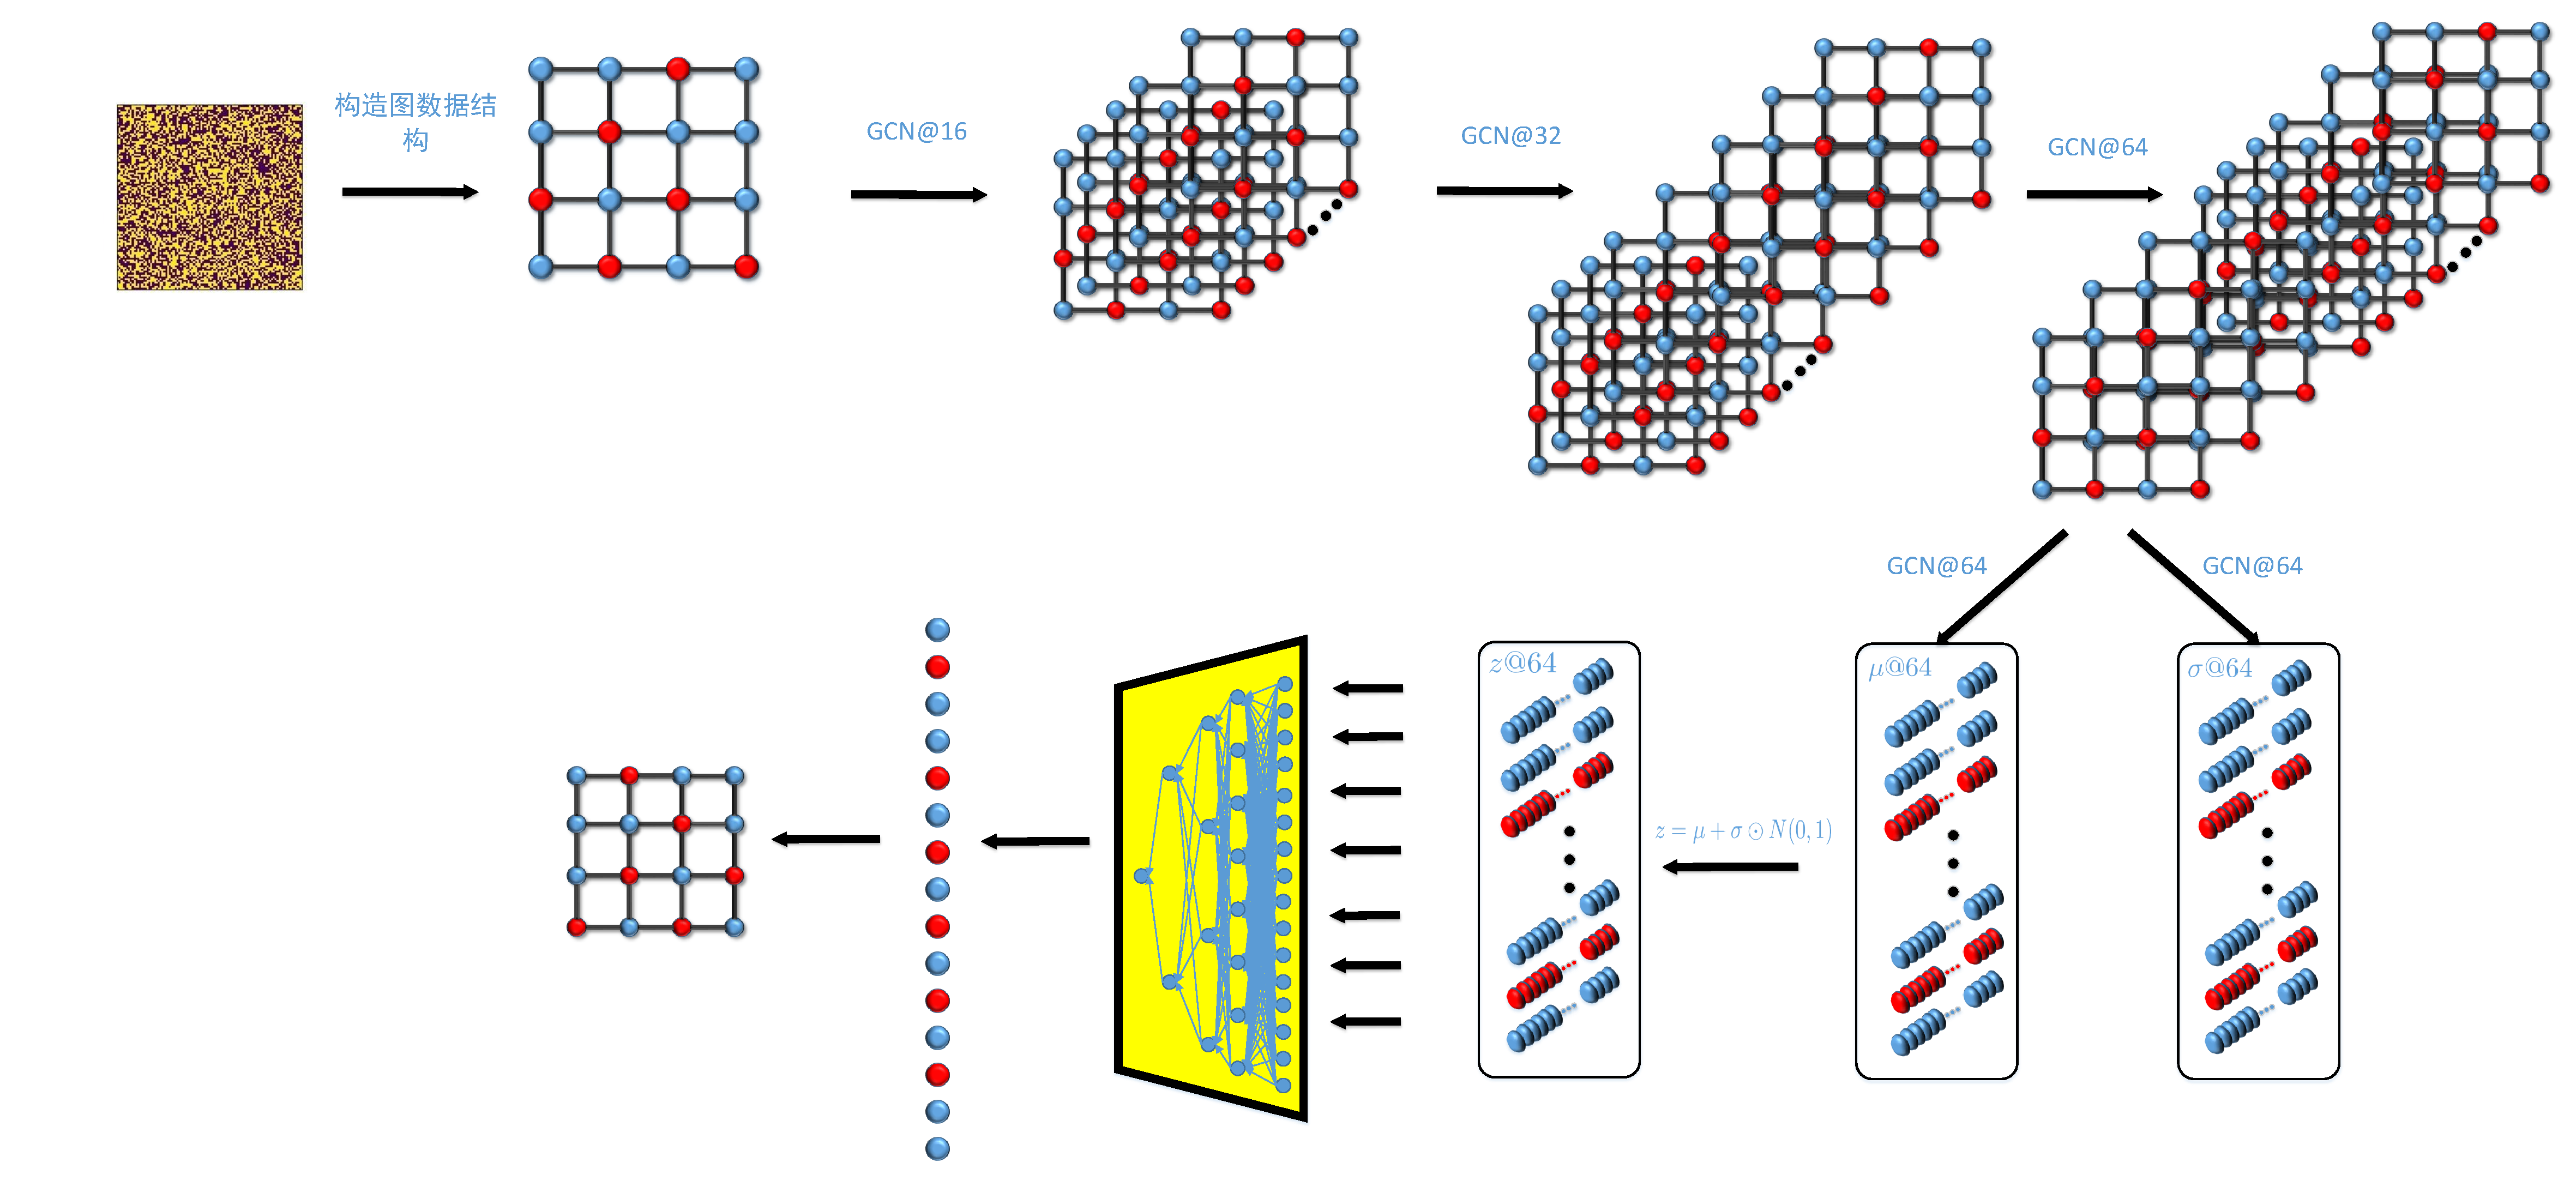
\includegraphics[scale=0.2]{spin_vgae2}
	\caption{\label{fig:wide}Use the figure* environment to get a wide figure that spans the page in \texttt{twocolumn} formatting.}
	\label{fig:spinvgae2}
\end{figure*}
		\begin{table*}
			\caption{\label{tab:table3}This is a wide table that spans the full page
				width in a two-column layout. It is formatted using the
				\texttt{table*} environment. It also demonstates the use of
				\textbackslash\texttt{multicolumn} in rows with entries that span
				more than one column.}
			\begin{ruledtabular}
				\begin{tabular}{ccccc}
					&\multicolumn{2}{c}{$D_{4h}^1$}&\multicolumn{2}{c}{$D_{4h}^5$}\\
					Ion&1st alternative&2nd alternative&lst alternative
					&2nd alternative\\ \hline
					K&$(2e)+(2f)$&$(4i)$ &$(2c)+(2d)$&$(4f)$ \\
					Mn&$(2g)$\footnote{The $z$ parameter of these positions is $z\sim\frac{1}{4}$.}
					&$(a)+(b)+(c)+(d)$&$(4e)$&$(2a)+(2b)$\\
					Cl&$(a)+(b)+(c)+(d)$&$(2g)$\footnotemark[1]
					&$(4e)^{\text{a}}$\\
					He&$(8r)^{\text{a}}$&$(4j)^{\text{a}}$&$(4g)^{\text{a}}$\\
					Ag& &$(4k)^{\text{a}}$& &$(4h)^{\text{a}}$\\
				\end{tabular}
			\end{ruledtabular}
		\end{table*}
		
		Insert an image using either the \texttt{graphics} or
		\texttt{graphix} packages, which define the \verb+\includegraphics{#1}+ command.
		(The two packages differ in respect of the optional arguments 
		used to specify the orientation, scaling, and translation of the image.) 
		To create an alignment, use the \texttt{tabular} environment. 
		
		The best place to locate the \texttt{figure} or \texttt{table} environment
		is immediately following its first reference in text; this sample document
		illustrates this practice for Fig.~\ref{fig:epsart}, which
		shows a figure that is small enough to fit in a single column. 
		
		In exceptional cases, you will need to move the float earlier in the document, as was done
		with Table~\ref{tab:table3}: \LaTeX's float placement algorithms need to know
		about a full-page-width float earlier. 
		
		Fig.~\ref{fig:wide}
		has content that is too wide for a single column,
		so the \texttt{figure*} environment has been used.%
		\begin{table}[b]
			\caption{\label{tab:table4}%
				Numbers in columns Three--Five are aligned with the ``d'' column specifier 
				(requires the \texttt{dcolumn} package). 
				Non-numeric entries (those entries without a ``.'') in a ``d'' column are aligned on the decimal point. 
				Use the ``D'' specifier for more complex layouts. }
			\begin{ruledtabular}
				\begin{tabular}{ccddd}
					One&Two&
					\multicolumn{1}{c}{\textrm{Three}}&
					\multicolumn{1}{c}{\textrm{Four}}&
					\multicolumn{1}{c}{\textrm{Five}}\\
					%\mbox{Three}&\mbox{Four}&\mbox{Five}\\
					\hline
					one&two&\mbox{three}&\mbox{four}&\mbox{five}\\
					He&2& 2.77234 & 45672. & 0.69 \\
					C\footnote{Some tables require footnotes.}
					&C\footnote{Some tables need more than one footnote.}
					& 12537.64 & 37.66345 & 86.37 \\
				\end{tabular}
			\end{ruledtabular}
		\end{table}
		
		The content of a table is typically a \texttt{tabular} environment, 
		giving rows of type in aligned columns. 
		Column entries separated by \verb+&+'s, and 
		each row ends with \textbackslash\textbackslash. 
		The required argument for the \texttt{tabular} environment
		specifies how data are aligned in the columns. 
		For instance, entries may be centered, left-justified, right-justified, aligned on a decimal
		point. 
		Extra column-spacing may be be specified as well, 
		although REV\TeX~4 sets this spacing so that the columns fill the width of the
		table. Horizontal rules are typeset using the \verb+\hline+
		command. The doubled (or Scotch) rules that appear at the top and
		bottom of a table can be achieved enclosing the \texttt{tabular}
		environment within a \texttt{ruledtabular} environment. Rows whose
		columns span multiple columns can be typeset using the
		\verb+\multicolumn{#1}{#2}{#3}+ command (for example, see the first
		row of Table~\ref{tab:table3}).%
		
		Tables~\ref{tab:table1}, \ref{tab:table3}, \ref{tab:table4}, and \ref{tab:table2}%
		\begin{table}[b]
			\caption{\label{tab:table2}
				A table with numerous columns that still fits into a single column. 
				Here, several entries share the same footnote. 
				Inspect the \LaTeX\ input for this table to see exactly how it is done.}
			\begin{ruledtabular}
				\begin{tabular}{cccccccc}
					&$r_c$ (\AA)&$r_0$ (\AA)&$\kappa r_0$&
					&$r_c$ (\AA) &$r_0$ (\AA)&$\kappa r_0$\\
					\hline
					Cu& 0.800 & 14.10 & 2.550 &Sn\footnotemark[1]
					& 0.680 & 1.870 & 3.700 \\
					Ag& 0.990 & 15.90 & 2.710 &Pb\footnotemark[2]
					& 0.450 & 1.930 & 3.760 \\
					Au& 1.150 & 15.90 & 2.710 &Ca\footnotemark[3]
					& 0.750 & 2.170 & 3.560 \\
					Mg& 0.490 & 17.60 & 3.200 &Sr\footnotemark[4]
					& 0.900 & 2.370 & 3.720 \\
					Zn& 0.300 & 15.20 & 2.970 &Li\footnotemark[2]
					& 0.380 & 1.730 & 2.830 \\
					Cd& 0.530 & 17.10 & 3.160 &Na\footnotemark[5]
					& 0.760 & 2.110 & 3.120 \\
					Hg& 0.550 & 17.80 & 3.220 &K\footnotemark[5]
					&  1.120 & 2.620 & 3.480 \\
					Al& 0.230 & 15.80 & 3.240 &Rb\footnotemark[3]
					& 1.330 & 2.800 & 3.590 \\
					Ga& 0.310 & 16.70 & 3.330 &Cs\footnotemark[4]
					& 1.420 & 3.030 & 3.740 \\
					In& 0.460 & 18.40 & 3.500 &Ba\footnotemark[5]
					& 0.960 & 2.460 & 3.780 \\
					Tl& 0.480 & 18.90 & 3.550 & & & & \\
				\end{tabular}
			\end{ruledtabular}
			\footnotetext[1]{Here's the first, from Ref.~\onlinecite{feyn54}.}
			\footnotetext[2]{Here's the second.}
			\footnotetext[3]{Here's the third.}
			\footnotetext[4]{Here's the fourth.}
			\footnotetext[5]{And etc.}
		\end{table}
		show various effects.
		A table that fits in a single column employs the \texttt{table}
		environment. 
		Table~\ref{tab:table3} is a wide table, set with the \texttt{table*} environment. 
		Long tables may need to break across pages. 
		The most straightforward way to accomplish this is to specify
		the \verb+[H]+ float placement on the \texttt{table} or
		\texttt{table*} environment. 
		However, the \LaTeXe\ package \texttt{longtable} allows headers and footers to be specified for each page of the table. 
		A simple example of the use of \texttt{longtable} can be found
		in the file \texttt{summary.tex} that is included with the REV\TeX~4
		distribution.
		
		There are two methods for setting footnotes within a table (these
		footnotes will be displayed directly below the table rather than at
		the bottom of the page or in the bibliography). The easiest
		and preferred method is just to use the \verb+\footnote{#1}+
		command. This will automatically enumerate the footnotes with
		lowercase roman letters. However, it is sometimes necessary to have
		multiple entries in the table share the same footnote. In this case,
		there is no choice but to manually create the footnotes using
		\verb+\footnotemark[#1]+ and \verb+\footnotetext[#1]{#2}+.
		\texttt{\#1} is a numeric value. Each time the same value for
		\texttt{\#1} is used, the same mark is produced in the table. The
		\verb+\footnotetext[#1]{#2}+ commands are placed after the \texttt{tabular}
		environment. Examine the \LaTeX\ source and output for
		Tables~\ref{tab:table1} and \ref{tab:table2}
		for examples.
		
		Video~\ref{vid:PRSTPER.4.010101} 
		illustrates several features new with REV\TeX4.2,
		starting with the \texttt{video} environment, which is in the same category with
		\texttt{figure} and \texttt{table}.%
		\begin{figure}	
			\centering
			\includegraphics[scale=0.15]{16mix_32_T_3}
			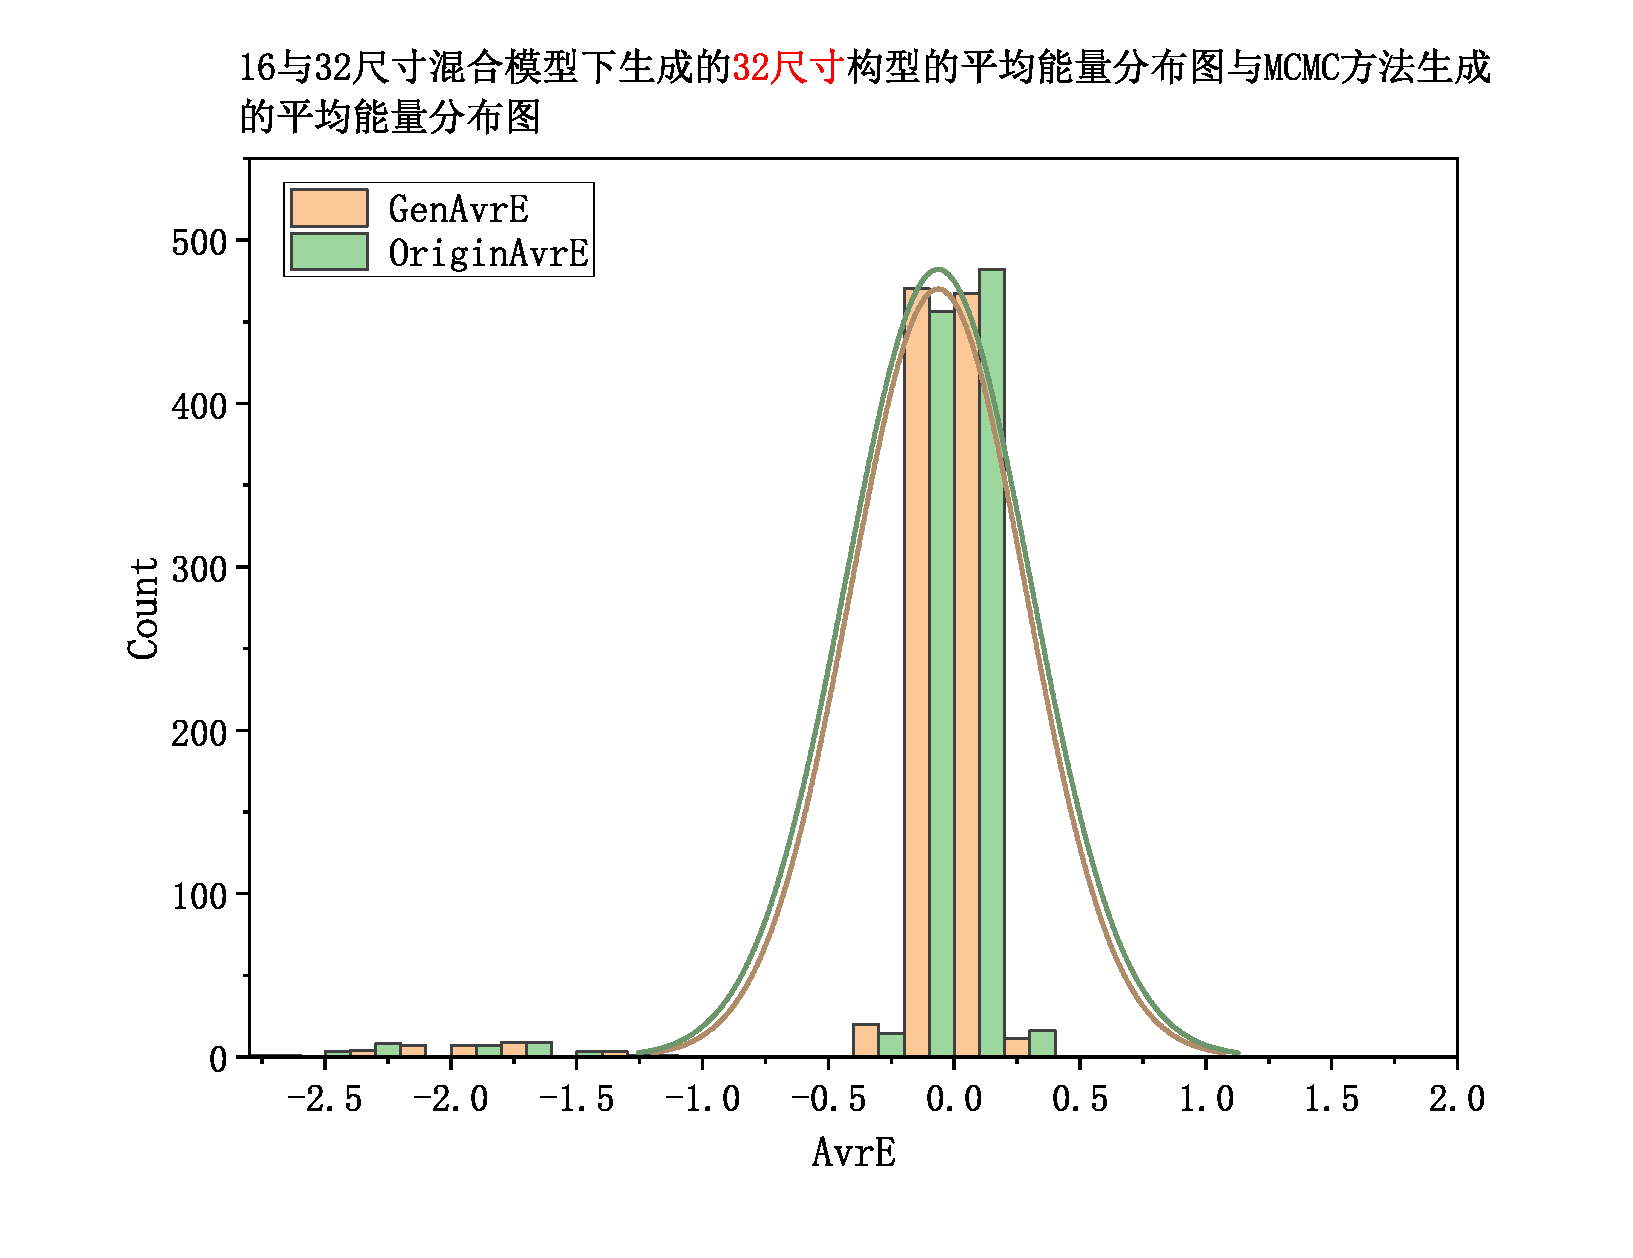
\includegraphics[scale=0.15]{16mix32_32_T_3}
			\caption{name of the figure} %  %大图名称
		%\label{fig:1}  %图片引用标记
		\end{figure}
		The \verb+\setfloatlink+ command causes the title of the video to be a hyperlink to the
		indicated URL; it may be used with any environment that takes the \verb+\caption+
		command.
		The \verb+\href+ command has the same significance as it does in the context of
		the \texttt{hyperref} package: the second argument is a piece of text to be 
		typeset in your document; the first is its hyperlink, a URL.
		
		\textit{Physical Review} style requires that the initial citation of
		figures or tables be in numerical order in text, so don't cite
		Fig.~\ref{fig:wide} until Fig.~\ref{fig:epsart} has been cited.
		
		\begin{acknowledgments}
			We wish to acknowledge the support of the author community in using
			REV\TeX{}, offering suggestions and encouragement, testing new versions,
			\dots.
		\end{acknowledgments}
		
		\appendix
		
		\section{Appendixes}
		
		To start the appendixes, use the \verb+\appendix+ command.
		This signals that all following section commands refer to appendixes
		instead of regular sections. Therefore, the \verb+\appendix+ command
		should be used only once---to setup the section commands to act as
		appendixes. Thereafter normal section commands are used. The heading
		for a section can be left empty. For example,
		\begin{verbatim}
			\appendix
			\section{}
		\end{verbatim}
		will produce an appendix heading that says ``APPENDIX A'' and
		\begin{verbatim}
			\appendix
			\section{Background}
		\end{verbatim}
		will produce an appendix heading that says ``APPENDIX A: BACKGROUND''
		(note that the colon is set automatically).
		
		If there is only one appendix, then the letter ``A'' should not
		appear. This is suppressed by using the star version of the appendix
		command (\verb+\appendix*+ in the place of \verb+\appendix+).
		
		\section{A little more on appendixes}
		
		Observe that this appendix was started by using
		\begin{verbatim}
			\section{A little more on appendixes}
		\end{verbatim}
		
		Note the equation number in an appendix:
		\begin{equation}
			E=mc^2.
		\end{equation}
		
		\subsection{\label{app:subsec}A subsection in an appendix}
		
		You can use a subsection or subsubsection in an appendix. Note the
		numbering: we are now in Appendix~\ref{app:subsec}.
		
		Note the equation numbers in this appendix, produced with the
		subequations environment:
		\begin{subequations}
			\begin{eqnarray}
				E&=&mc, \label{appa}
				\\
				E&=&mc^2, \label{appb}
				\\
				E&\agt& mc^3. \label{appc}
			\end{eqnarray}
		\end{subequations}
		They turn out to be Eqs.~(\ref{appa}), (\ref{appb}), and (\ref{appc}).
		
		% The \nocite command causes all entries in a bibliography to be printed out
		% whether or not they are actually referenced in the text. This is appropriate
		% for the sample file to show the different styles of references, but authors
		% most likely will not want to use it.
		\nocite{*}
		\bibliographystyle{plain}
		\bibliography{apssamp}% Produces the bibliography via BibTeX.
		
	\end{document}